\documentclass{article}
\usepackage[utf8]{inputenc}
\usepackage[T1]{fontenc}
\usepackage{geometry}[margin=2cm]
\usepackage{float}
\usepackage{lmodern}

\usepackage{amsmath}
\usepackage{amssymb}
\usepackage{amsthm}
\usepackage{enumerate}
\usepackage{mathtools}
\usepackage[]{algorithm2e}

\usepackage{xcolor}
\usepackage{listings}
\lstset{language=Matlab, texcl=true, backgroundcolor=\color{yellow!3},
	frame=single, rulecolor=\color{yellow!3}, framesep=8pt, numbers=left}

\newcommand{\bR}{\mathbb{R}}
\newcommand{\bC}{\mathbb{C}}
\newcommand{\cL}{\mathcal{L}}
\newcommand{\cM}{\mathcal{M}}

\DeclareMathOperator{\diag}{diag}
\DeclareMathOperator{\Id}{Id}

\begin{document}
	\begin{center}
		{\huge Tarea \#2}\par
		Análisis Numérico MA0501\par\vskip1ex
		Isaac Chaves Arguedas\quad A71841\\
		Jorge Andrés Ramos García\quad B65792\\
		Kevin Rojas Cisneros\quad B76661\\
		Andrés Zamora Nasralah\quad B78534
	\end{center}

	\section*{Ejercicio 1}
	\input{ejer01}
	\section*{Ejercicio 2}
	\paragraph{(a)}
\paragraph{(b)}
\paragraph{(c)}

Sea $A\in\bC^{m\times n}$ ($m\geq n$), $A=U\Sigma V^*$ una descomposición en valores singulares de $A$, donde $\Sigma\in\bC^{m\times n}$. Sea $J\in\bC^{m\times n}$ la matriz con 1's en la diagonal principal, es decir, $J_{ij}=\delta_{ij}$ (no es necesariamente cuadrada). Como los elementos de la diagonal principal de $\Sigma$ son no negativos (y el resto de elementos on 0), entonces para todo $\epsilon>0$ la matriz $\Sigma+\epsilon J$ es de rango completo.

Defina la sucesión
\[
	A_k=U\left(\Sigma+\frac{1}{k}J\right)V^*
\]
que está conformada por matrices de rango completo. Así
\[
	\Vert A_k-A\Vert_2=\frac{1}{k}\Vert UJV^*\Vert_2\to0
	\quad\text{cuando }k\to\infty
\]

Por tanto, $A$ es límite de matrices de rango completo. Se concluye que el conjunto de matrices de rango completo es denso en $\bC^{m\times n}$.
	\section*{Ejercicio 3}
	\paragraph{(a)}
Definimos $f(x)=\tan(x)-\sin(x)$, redondeando a 4 decimales
	\begin{footnotesize}
	\begin{center}\begin{tabular}{|c||c|c|c|}\hline
			$x$    & $\quad{}0.91153\quad{}$& $\quad{}1.08265\quad{}$ & $\quad{}1.17959\quad{}$\\ \hline
			$f(x)$ &$0.5000$ &$1.0000$ &$1.5000$ \\ \hline
	\end{tabular}\end{center}
\end{footnotesize}
\paragraph{(b)}
Construimos el polinomio de Lagrange de grado 2 para aproximar $f^{-1}$ utilizando los puntos anteriores:
\begin{align*}
p_2(x)&=0.91153\cdot\frac{(x-1)(x-1.5)}{(0.5-1)(0.5-1.5)}+1.08265\cdot\frac{(x-0.5)(x-1.5)}{(1-0.5)(1-1.5)}+1.17959\cdot\frac{(x-0.5)(x-1)}{(1.5-0.5)(1.5-1)}\\
&= 0.91153(2x^2-5x+3)-1.08265(4x^2-8x+3)+1.17959(2x^2-3x+1)\\
&=-0.14836x^2+0.56478x+0.66623
\end{align*}
\paragraph{(c)}
Encontrar una soluci\'on aproximada a la ecuaci\'on $f(x)=0.436$ es equivalente a aproximar la imagen de $0.436$ bajo $f^{-1}$, as\'i, aproximando $f^{-1}$ con $p_2$ obtenemos
$$p_2(0.436)=0.8842714374...$$
Usando como soluci\'on exacta $\xi:=0.8783933784...$ vemos f\'acilmente que la aproximaci\'on tiene un d\'igito decimal correcto. Adem\'as el error relativo es aproximadamente:
$$\frac{|p_2(0.436)-\xi|}{|\xi|}\approx\frac{|0.8842714374-0.8783933784|}{|0.8783933784|}=\frac{0.0058780590}{0.8783933784}\approx0.00669182981$$
y note que:
$$5\cdot10^{-3}<0.00669182981<5\cdot 10^{-2}$$
por lo que tenemos dos d\'igitos significativos.

	\section*{Ejercicio 4}
	Según se estudió en clase\footnote{Ver también \emph{Numerical Analysis} de R. Burden \& D. Faires, sección sobre interpolación por \emph{splines} cúbicos naturales.}, debemos resolver el sistema $Ax=y$ para encontrar los coeficientes $a_i,b_i,c_i,d_i$, donde
\begin{align*}
	A&=
	\begin{bmatrix}
		1 & 0 & 0 & 0 \\
		h_0 & 2(h_0+h_1) & h_1 & 0 \\
		0 & h_1 & 2(h_1+h_2) & h_2 \\
		0 & 0 & 0 & 1
	\end{bmatrix}\\
	y& = 3
	\begin{bmatrix}
		0\\
		\frac{1}{h_1}(a_2-a_1)-\frac{1}{h_0}(a_1-a_0)\\
		\frac{1}{h_2}(a_3-a_2)-\frac{1}{h_1}(a_2-a_1)\\
		0
	\end{bmatrix}\\
	x&=(c0,c1,c2,c3)^t\\
	h_i&=x_{i+1}-x_{i},\quad i=0,1,2\\
	a_i&=y_i=f(x_i),\quad i=0,1,2,3\\
	b_i&=\frac{1}{h_i}(a_{i+1}-a_i)-\frac{h_i}{3}(2c_i+c_{i+1})\\
	d_i&=\frac{1}{3h_i}(c_{i+1}-c_i)
\end{align*}

Como $c_0=c_3=0$, basta resolver el sistema
\[
	\begin{bmatrix}
		4h & h \\
		h & 4h
	\end{bmatrix}
	\begin{bmatrix}
		c_1\\
		c_2
	\end{bmatrix}
	=
	\frac{3}{h}
	\begin{bmatrix}
		a_2+a_0-2a_1\\
		a_3+a_1-2a_2
	\end{bmatrix}
\]
Note que $h_i=h=0.25$. Sustituyendo $h$ y reacomodando:
\[
\frac{1}{12}
\begin{bmatrix}
1 & 1/4 \\
1/4 & 1
\end{bmatrix}
\begin{bmatrix}
c_1\\
c_2
\end{bmatrix}
=
\begin{bmatrix}
a_2+a_0-2a_1\\
a_3+a_1-2a_2
\end{bmatrix}
\]
Si se resuelve este sistema en MATLAB, se obtiene que $c_1\approx59.1967224132176$ y $c_2\approx100.2945081600630$.

Ahora aproximo el valor de $f(2.65)$. Puesto que $2.5<2.65<2.76$ entonces debemos emplear el polinomio del tercer subintervalo, $s_2(x)=a_2+b_2(x-x_2)+c_2(x-x_2)^2+d_2(x-x_2)^3$. Usando las fórmulas anteriores,
\begin{align*}
	a_2&\approx79.186210744572577\\
	b_2&\approx120.1757303031561\\
	c_2&\approx100.2945081600630\\
	d_2&\approx-133.7260108800840
	\intertext{y entonces}
	s_2(2.65)&\approx99.017871436927123
\end{align*}

El valor que se obtiene en una calculadora es $f(2.65)\approx98.370568585361809$. El error es $|s_2(2.65)-f(2.65)|\approx0.647302851565314$ y el error relativo es
\[
	\frac{|s_2(2.65)-f(2.65)|}{|f(2.65)|}\approx0.006580249162671
\]

	\section*{Ejercicio 5}
	\paragraph{(a)}
Sea $F:\mathbb{R}^n\longrightarrow\mathbb{R}^n$. Suponga que $F(c)=0$, $J_F(c)$ es invertible y $F\in C^2(V)$ para $V$ un vecindario de $c$, queremos mostrar que para una selecci\'on de $x_0$ inicial suficientemente cerca de $c$ la iteraci\'on del m\'etodo de Newton converge a $c$.
Considere la función:
$$g(x)=x-(J_F(x))^{-1}F(x)$$
$g$ tiene un punto fijo en $c$. Como $F$ es clase $C^2$, $g$ es clase $C^1$ y tiene sentido considerar $J_g(x)$.
Veamos que $J_g(c)=0_{nxn}$ pues:\\
Si $h(x)=(J_F(x))^{-1}F(x)=(h_i(x))_{1\leq i \leq n}$,  $[J_F(x)]^-1=(a_{ij}(x))_{1\leq i,j \leq n}$, $J_h(x)=(b_{ij}(x))_{1\leq i,j \leq n}$, entonces:
$$h_i(x)=\sum_{k=1}^{n}a_{ik}(x)F_k(x)$$ y
$$b_{ij}(x)=\dfrac{\partial c_i}{\partial x_j}(x)=\sum_{k=1}^{n}\dfrac{\partial a_{ik}}{\partial x_j}(x)F_k(x)+\sum_{k=1}^{n}a_{ik}(x)\dfrac{\partial F_k(x)}{\partial x_j}$$
Note que al evaluar en $c$ la primera sumatoria se anula pues $F(c)=0$. Además como $\dfrac{\partial F_k(x)}{\partial x_j}(c)$ es la $(k,j)$-\'esima entrada de $J_F(c)$ entonces $$J_h(c)=[J_F(c)]^{-1}\cdot J_F(c)=I_{nxn}$$. Luego $J_g(c)=0_{nxn}$.
Adem\'as existe $\epsilon>0$ tal que si $\overline{B}_\epsilon(c)\subset V$ es la bola cerrada de radio $\epsilon$ alrededor de $c$, entonces 
$$\|J_g(x)\|_\infty<0.5,\ \forall x\in\overline{B}_\epsilon(c)$$
Dados $x,y\in\bar{B_\epsilon}(c)$, por Teorema del valor medio existe $\eta\in(0,1)$ tal que 
$$g_i(x)-g_i(y)=\nabla g_i(\eta x+(1-\eta)y)\cdot(x-y)=\sum_{k=1}^{n}(x_j-y_j)\dfrac{\partial g_i}{\partial x_j}(\eta x + (1-\eta)y)$$.
Adem\'as como $|x_j-y_j|\leq\|x-y\|_\infty$ y $\|J_g(z)\|_\infty=\underset{1\leq i\leq n}{\max}\sum_{k=1}^{n}\left |\dfrac{\partial g_i}{\partial x_j}\right|$. Entonces
$$|g_i(x)-g_i(y)|\leq\|x-y\|_\infty\|J_g(\eta x+(1-\eta)y)\|_\infty,\ \forall i=1,...,n$$.
Ahora, si $x,y\in\overline{B}_\epsilon(c)$ tenemos:
$$\|g(x)-g(y)\|_\infty\leq 0.5\|x-y\|_\infty$$
Finalmente, si tomamos $y=c$ entonces tenemos que
$$\|g(x)-c\|_\infty < \|x-c\|_\infty,\ \forall x\in\overline{B}_\epsilon(c)$$
Luego, $g(\overline{B}_\epsilon(c))\subseteq\overline{B}_\epsilon(c)$, y se tiene que la sucesi\'on dada por $x^{(k)}=g(x^{(k-1)})$ converge a al \'unico punto fijo de $g$ en $\overline{B}_\epsilon(c)$ para cualquier selecci\'on de $x^{(0)}\in\overline{B}_\epsilon(c)$ incial, es decir, la iteraci\'on de Newton converge al cero de $F$. Para obtener la convergencia cuadr\'atica, considere el polinomio de Taylor para $F$ centrado en $x^{(k)}$:
$$0=F(c)=F(x^{(k)})+J_F(x^{(k)})(c-x^{(k)})+\frac{1}{2}E_F$$
donde $E_F$ incluye los t\'erminos de las segundas derivadas as\'i,
$$\|E_F\|_\infty\leq n^3A\|c-x^{(k)}\|^2_\infty$$
donde el t\'ermino $A:=\underset{1\leq i,j,l}{\max}\underset{x\in\overline{B}_\epsilon(c)}{\max}\left |\dfrac{\partial^2 F_i}{\partial x_j \partial x_l}(x)\right |$, el t\'ermino $n^3$ es de todas las combinaciones de $i,j,l$. Luego, de la expansi\'on de Taylor se obtiene
$$x^{(k+1)}-c=x^{(k)}-c-[J_F(x^{(k)})]^{-1}f(x^{(k)})=\frac{1}{2}[J_F(x^{(k)})]^{-1}E_F$$
y as\'i, si $C:=\underset{x\in\overline{B}_\epsilon(c)}{\max}\|[J_F(x)]^{-1}\|_\infty^2$, entonces
$$\|x^{(k+1)}-c\|_\infty\leq\frac{1}{2}n^3CA\|x^{(k)}-c\|_\infty^2$$.
De lo que se deduce que la convergencia es cuadr\'atica.
\paragraph{(b)}
Dado el sistema no lineal:
$$
\begin{cases}
3x_1 \ - \ \cos(x_2 x_3) = 0.5,\\
x_1^2 \ - \ 81(x_2+0.1)^2 \ + \ \sin(x_3) = -1.06,\\
e^{-x_1 x_2} \ + \ 20x_3 = \frac{3-10\pi}{3}
\end{cases}
$$
podemos reescribir el sistema por $f_1(x_1,x_2,x_3)=0$, $f_2(x_1,x_2,x_3)=0$,\\ $f_3(x_1,x_2,x_3)=0$ donde:
\begin{align*}
f_1(x_1,x_2,x_3)&=3x_1-\cos(x_2 x_3)-0.5,\\
f_2(x_1,x_2,x_3)&=x_1^2-81(x_2+0.1)^2+\sin(x_3)+1.06,\\
f_3(x_1,x_2,x_3)&=e^{-x_1 x_2}+20x_3-\dfrac{3-10\pi}{3}.
\end{align*}
\paragraph{(c)}
La iteraci\'on de Newton para el sistema anterior viene dada por:
$$\textbf{x}^{(k+1)} = \textbf{x}^{(k)} - \left[ J(\textbf{x}^{(k)}) \right]^{-1} \textbf{F}(\textbf{x}^{(k)})$$
Donde $\textbf{F}$ es la funci\'on definida por el sistema, a la que se le desea hallar un cero:
$$\textbf{F}(\textbf{x})=\textbf{F}(x_1,x_2,x_3)=\begin{pmatrix}
3x_1-\cos(x_2x_3)-0.5\\
x_1^2-81(x_2+0.1)^2+\sin(x_3)+1.06\\
e^{-x_1x_2}+20x_3-\frac{3-10\pi}{3}
\end{pmatrix}$$
y $J$ es la matriz Jacobiana de $\textbf{F}$, explicitamente:
$$J(x)=J(x_1,x_2,x_3)=
\begin{pmatrix}
3&x_3\sin(x_2 x_3)&x_2\sin(x_2x_3)\\
2x_1&-162x_2-\frac{81}{5}&\cos(x_3)\\
-x_2 e^{-x_1x_2}&-x_1 e^{-x_1x_2}&20
\end{pmatrix}
$$
\paragraph{(d)}
Aplicando la funci\'on en \textbf{(f)} para aproximar la soluci\'on al sistema tras 3 iteraciones del m\'etodo de Newton con $x^{(0)}=[0.1,0.1,-0.1]^t$ obtenemos:
$$x^{(1)}\approx[0.4998696729,0.0194668485,-0.5215204719]^t$$
$$x^{(2)}\approx[0.5000142402,0.0015885914,-0.5235569643]^t$$
$$x^{(3)}\approx[0.5000001135,0.0000124448,-0.5235984501]^t$$
\paragraph{(e)}
El algoritmo para del m\'etodo de Newton es el siguiente:
\begin{algorithm}
	\KwIn{\\F: Funci\'on clase $C^1$\\
		$x_0$: Aproximaci\'on inicial\\
		tol: Tolerancia\\
		itermax: M\'ximo de iteraciones}
	\KwOut{Aproximaci\'on $x_k$ de la ra\'iz de F}
	$k=1$;\\
	$J=jacobian(F)$;\\
	$err=||F(x_0)||$;\\
	\While{$k\leq itermax\ \&\&\ err>tol$}{
		$y_k=J(x_{k-1})\backslash(-F(x_{k-1}))$;\\
		$x_k=x_{k-1}+y_k$;\\
		$k=k+1$;\\
		$err=||F(x_k)||$;
	}
	\caption{Algoritmo de Newton}
\end{algorithm}
\paragraph{(f)}.
\lstinputlisting[language=MatLab]{Ejercicio5.m}

	\section*{Ejercicio 6}
	\paragraph{(a)}
Sea $f\colon\bC^{2m}\to\bC$ dada por $f(x,y)=x^*y$ (nota: el enunciado dice $x^ty$, que no es exactamente el producto interno en $\bC$, pero la demostración es la misma). El algoritmo $\tilde{f}:\mathbb{F}^{2m}\to\mathbb{F}$ de producto interno está dado por
\[
	\tilde{f}(x,y)=fl\left(\sum_{k=1}^m fl(\bar{x}_ky_k)\right)
\]

Dados $x,y\in\bC^m$, existen $\epsilon_1,\dotsc,\epsilon_m$ con $|\epsilon_k|\leq\epsilon_{m\'aq}$, donde $\epsilon_{m\'aq}$ es el épsilon de la máquina, tales que $fl(\bar{x}_ky_k)=\bar{x}_ky_k(1+\epsilon_k)$. Además, existe $\epsilon_{m+1}$ con $|\epsilon_{m+1}|\leq\epsilon_{m\'aq}$ tal que
\[
	fl\left(\sum_{k=1}^m fl(\bar{x}_ky_k)\right)=\left(\sum_{k=1}^m fl(\bar{x}_ky_k)\right)(1+\epsilon_{m+1})
\]
Combinando lo anterior, obetenemos que
\[
	\tilde{f}(x,y)=\sum_{k=1}^m \bar{x}_ky_k(1+\epsilon_{k})(1+\epsilon_{m+1})
\]
y el error es
\begin{align*}
	|\tilde{f}(x,y)-f(x,y)|&=\left|\sum_{k=1}^m \bar{x}_ky_k(\epsilon_{k}+\epsilon_{m+1}+\epsilon_k\epsilon_{m+1})\right|\\
	&\leq\Vert x\Vert_2\left(\sum_{k=1}^m|y_k|^2\,|\epsilon_k+\epsilon_{m+1}+\epsilon_k\epsilon_{m+1}|^2\right)^{\frac{1}{2}}&\text{(desig. Cauchy-Schwartz)}\\
	&\leq\Vert x\Vert_2\left(\sum_{k=1}^m|y_k|^2\,(|\epsilon_k|+|\epsilon_{m+1}|+|\epsilon_k\epsilon_{m+1}|)^2\right)^{\frac{1}{2}}\\
	&\leq\Vert x\Vert_2\left(\sum_{k=1}^m|y_k|^2\,(2|\epsilon_{m\'aq}|+|\epsilon_{m\'aq}|^2)^2\right)^{\frac{1}{2}}\\
	&=\Vert x\Vert_2\Vert y\Vert_2(2|\epsilon_{m\'aq}|+|\epsilon_{m\'aq}|^2)
\end{align*}
de manera que
\[
	\frac{|\tilde{f}(x,y)-f(x,y)|}{\Vert x\Vert_2\Vert y\Vert_2}\leq 2|\epsilon_{m\'aq}|+|\epsilon_{m\'aq}|^2=O(\epsilon_{m\'aq})
\]

Dados $x,y\in\bC^{m}\setminus\{0\}$, existe $i$ tal que $\sqrt{m}|x_i|\geq\Vert x\Vert_2$ (precisamente, $i$ tal que $|x_i|=\Vert x\Vert_\infty$). Defina $\tilde{x},\tilde{y}$ dados por
\begin{align*}
	\tilde{x}_k&=x_k\qquad\forall k=1,\dotsc,m\\[1ex]
	\tilde{y}_k&=y_k\qquad k\neq i\\[1ex]
	\tilde{y}_i&=
		\frac{1}{\bar{x}_i}\Bigl(\tilde{f}(x,y)-\sum_{l\neq i}\bar{x}_ly_l\Bigr)
\end{align*}
note que evidentemente $f(\tilde{x},\tilde{y})=\tilde{f}(x,y)$. Vea que el error entre $\tilde{y}$ y $y$ es igual a
\[
	\frac{\Vert \tilde{y}-y\Vert_2}{\Vert y\Vert_2} =\frac{|\tilde{y}_i-y_i|}{\Vert y\Vert_2} =\frac{|\tilde{f}(x,y)-f(x,y)|}{|x_i|\Vert y\Vert_2}
	\leq\sqrt{m}\frac{|\tilde{f}(x,y)-f(x,y)|}{\Vert x\Vert_2\Vert y\Vert_2} =O(\epsilon_{m\'aq})
\]

Claramente $\dfrac{\Vert\tilde{x}-x\Vert_2}{\Vert x\Vert_2}=0=O(\epsilon_{m\'aq})$.

\smallskip
$\therefore$ El algoritmo $\tilde{f}$ es estable para atrás.
\paragraph{(b) Efectos del factor de crecimiento:}
\subparagraph{(a)} \strut

\lstinputlisting{../codigo/matrizPatologica.m}

\subparagraph{(b)} Al correr el siguiente código
\lstinputlisting[numbers=none]{../codigo/ejer6bb.m}
se obtuvo que el factor de crecimiento es aproximadamente $5.629\times10^{14}$ y la norma es $0$.

Es fácil notar que la descomposición $LU$ de $A$ está dada por
\[
	L=\begin{bmatrix}
		1      & 0      & 0      & \cdots & 0      \\
		-1     & 1      & 0      & \cdots & 0      \\
		-1     & -1     & 1      & \cdots & 0      \\
		\vdots & \vdots & \vdots & \ddots & \vdots \\
		-1     & -1     & -1     & \cdots & 1
	\end{bmatrix}
	\quad\text{y}\quad
	U = \begin{bmatrix}
		1      & 0      & 0      & \cdots & 0      & 1      \\
		0      & 1      & 0      & \cdots & 0      & 2      \\
		0      & 0      & 1      & \cdots & 0      & 4      \\
		\vdots & \vdots & \vdots & \ddots & \vdots & \vdots \\
		0      & 0      & 0      & \cdots & 1      & 2^{48} \\
		0      & 0      & 0      & \cdots & 0      & 2^{49}
	\end{bmatrix}
\]
y vemos que $\rho(A)=2^{49}\approx5.629\times10^{14}$, que es el resultado que habíamos obtenido antes.

Recuerde que la aritmética de precisión doble puede representar de manera exacta potencias de 2 hasta $2^{1023}$, por lo que la matriz $U$ es almacenable de forma exacta. Al calcular el producto $LU$ el peor caso posible sucede al calcular la esquina inferior derecha, se debe realizar la sumatoria
\[
	-1-2-4-8-\dotsb-2^{48}+2^{49}
\]
que la computadora calcula asociando a la izquierda, y puesto que en ningún paso de esta sumatoria, el número es una potencia de 2, es posible que haya errores de redondeo. Sin embargo, recuerde también que la precisión doble posee 53 dígitos significativos (52 dígitos de mantisa más un dígito de parte entera), mientras que el número $-1-2-4-\dotsb-2^{48}$ tiene 49 dígitos significativos, por lo que es posible almacenarlo de forma exacta. Al sumar el último término $2^{49}$, el cálculo requiere de un registro con por lo menos 50 bits, que existe pues hay 53 dígitos disponibles (algunos procesadores realizan las operaciones aritméticas en registros de mayor tamaño, y luego redondean a precisión doble).

De hecho, el número mayor de $m$ posible para que no haya error de redondeo es $m=54$. La razón de esto es que el número
\[
	-1-2-4-8-\dotsb-2^{52}
\]
tiene 53 cifras significativas, que es el mayor caso almacenable de forma exacta. Al sumar el último término $2^{53}$, si el procesador es adecuado, la operación se realiza en un registro de mayor tamaño, y entonces se calcula de forma exacta. Este es el caso en una computadora personal moderna cualquiera. En efecto, si se corre el programa anterior con $m=54$, no hay error, pero al correrlo con $m=55$, el error es $\Vert A-LU\Vert_2=1$.

\subparagraph{(c)} El siguiente código genera el gráfico.
\lstinputlisting[numbers=none]{../codigo/ejer6bc.m}

\begin{figure}[H]
	\centering
	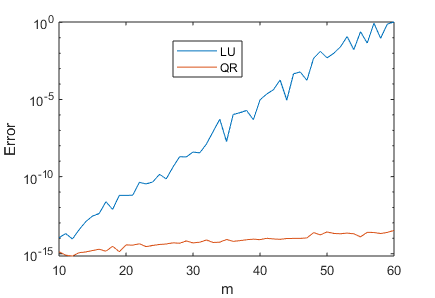
\includegraphics{ejer6bc.png}
	\caption{Comparación de los errores usando las descomposiciones QR y LU.}
\end{figure}

El error usando la descomposición $LU$ crece muchísimo más rápido que el de $QR$. Sabemos que la matriz $U$ tiene entradas que crecen del orden de $2^{m}$, por lo que su factor de crecimiento $\rho$ y el error en la resolución de ecuaciones también crecen exponencialmente.

Por otro lado, el error de resolver sistemas emplenado la factorización $QR$ depende del número de condición, precisamente, el error es del orden $O(\kappa(A)\epsilon_{m\'aq})$ (un resultado visto en clase). Hay que obtener $\kappa(A)=\Vert A\Vert_\infty\Vert A^{-1}\Vert_\infty$. Un cálculo nos dice que
\[
	A^{-1}=
	\begin{bmatrix}
		\frac{1}{2} & -\frac{1}{4} & -\frac{1}{8} & \cdots & -\frac{1}{2^{m-1}} & -\frac{1}{2^{m-1}}     \\[2pt]
		0           & \frac{1}{2}  & -\frac{1}{4} & \cdots & -\frac{1}{2^{m-2}} & -\frac{1}{2^{m-2}} \\[2pt]
		0           & 0            & \frac{1}{2}  & \cdots & -\frac{1}{2^{m-3}} & -\frac{1}{2^{m-3}} \\[2pt]
		\vdots      & \vdots       & \vdots       & \ddots & \vdots             & \vdots             \\[2pt]
		0           & 0            & 0            & \cdots & \frac{1}{2}        & -\frac{1}{2}       \\[2pt]
		\frac{1}{2} & \frac{1}{4}  & \frac{1}{8}  & \cdots & \frac{1}{2^{m-1}}  & \frac{1}{2^{m-1}}
	\end{bmatrix}
\]
(el patrón se sigue en las primeras $m-1$ columnas, y se rompe en la última). Puede verificar que esta es la inversa realizando el producto $AA^{-1}$. Como la norma-$\infty$ de matrices es el máximo de las normas-$1$ de cada fila, y como la norma-1 de cada fila es precisamente 1, entonces vemos que $\Vert A^{-1}\Vert_\infty=1$. Por otro lado, se calcula fácilmente que $\Vert A\Vert_\infty=m$. Por tanto $\kappa(A)=m$, es decir, el número de condición condición crece linealmente. Esto justifica que el error empleando la descomposición $QR$ sea mucho menor que aquel de emplear la descomposición $LU$.
	\section*{Ejercicio 7}
	\paragraph{(a)}
El An\'alisis de Componentes Principales (PCA) consiste en una transformaci\'on lineal ortogonal que transforma los datos
a un nuevo sistema coordenado de tal forma que este nuevo sistema queda determinado por \textit{componentes principales}
que est\'an no correlacionados entre s\'i (son ortogonales), pero que tienen m\'axima correlaci\'on con las mediciones.
Esta transformaci\'on consigue que el primer componente principal tenga la mayor posible varianza, el siguiente componente segunda
mayor varianca y as\'i sucesivamente. Para esto, los datos se pre-procesan y luego se ejecuta SVD. 
\\
M\'as espec\'ificamente, suponiendo que $X$ es una matriz que contiene en cada fila mediciones de un experimento y que al cambiar de fila
lo que cambia es el \textit{feature} del experimento, calculamos la media $\bar{x}$ como 
\[\bar{x}_j = \frac{1}{n}\sum_{i=1}^nX_{ij} \]
y la matriz promedio la definimos como 
\[\bar{X} = h\cdot\bar{x}^t \]
donde $h$ es un vector que cumple $h_i = 1$ para $i=1,\ldots,n$. Se define la matriz promedio-substra\'ida $B$ como
\[ B = X-\bar{X} \]
y la matriz de covarianca de las filas de $B$ es dada por
\[ C = \frac{1}{n-1}B^*B \]

Con esto, la relaci\'on entre PCA y SVD se puede visualizar m\'as claramente: el componente principal $u_1$ es dado por
\[ u_1 = \arg \max_{||u_1||=1} u_1^*B^*Bu_1 \]
el cual corresponde al vector propio de $B^*B$ correspondiente al mayor valor propio. De aqu\'i es claro que $u_1$ es el vector singular 
izquierdo de $B$ correspondiente al m\'as grande valor singular. Luego, los componentes principales se 
encuentran  aplicando descomposici\'on por valores propios a la matriz $C$.\\
\paragraph{(b)}
Se eligi\'o el ejemplo de \textit{Ovarian cancer data}. La idea del ejemplo es estudiar la informaci\'on
gen\'etica de 216 pacientes, de los cuales 121 tienen c\'ancer de ovario y 95 no. Para cada paciente
hay un vector de datos que contiene la expresi\'on gen\'etica de 4000 genes. Los datos de expresi\'on gen\'etica tienen la complejidad de ser de alta dimensi\'on (aqu\'i, dimensi\'on se refiere a la cantidad de 
atributos que un conjunto de datos tiene). Una sola persona tiene millones de posibles combinaciones gen\'eticas y esto provoca
que la informaci\'on gen\'etica de los pacientes tengan alta correlaci\'on, al punto que la informaci\'on de un paciente se traslapa
con otros. Para poder visualizar patrones y correlaciones
en datos de alta dimensi\'on como \'estos el uso de PCA se vuelve fundamental.\\
\paragraph{(c)}
El c\'odigo se muestra a continuaci\'on.
\lstinputlisting[language=MATLAB]{../codigo/ejer7.m}
El resultado que se obtiene es el gr\'afico de la siguiente figura.
\begin{figure}[H]
   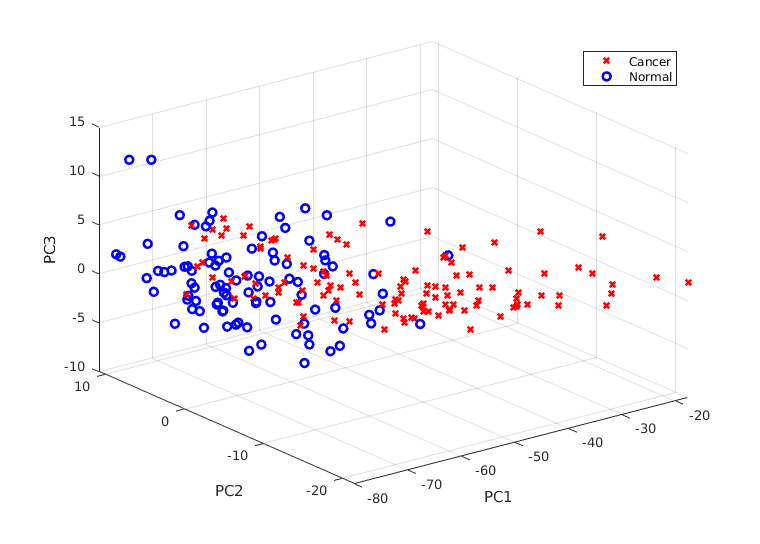
\includegraphics[width=\textwidth]{ejer7c.png}
   \centering
   \caption{Gr\'afico usando PCA en datos de pacientes con c\'ancer y pacientes sanos.}
\end{figure}

Se observa que los datos de  personas con c\'ancer tienden a dispersarse m\'as que las personas sin c\'ancer.

	
\end{document}